\documentclass[a4paper,11pt,leqno,notitlepage,onecolumn]{article}
%\documentclass[a4paper,11pt,leqno,notitlepage,twocolumn]{article}

\usepackage[latin1]{inputenc}
\usepackage{fontenc}
\usepackage{graphicx}
\usepackage[dvips]{hyperref}
\usepackage{subfigure}
\usepackage{setspace}
%\doublespacing
\usepackage[a4paper]{geometry}
\geometry{top=1in, bottom=1in, left=1in, right=1in}

\begin{document}
\title{PIX: PMaC's Efficient Binary Instrumentor for Linux on x86 Platforms}
\author{Michael Laurenzano, Mustafa M. Tikir, Laura Carrington, Allan Snavely\\
San Diego Supercomputer Center\\
9500 Gilman Drive, La Jolla, CA 92037\\
\it{\{michaell,mtikir,laurac,allans\}@sdsc.edu}}
\date{}
\maketitle

\begin{abstract}
\begin{it}

Binary instrumentation enables insertion of additional code into an
executable in order to observe or modify the behavior of application runs. 
There are two main approaches to binary instrumentation: static and dynamic
binary instrumentation. In this paper, we present PMaC's instrumentation toolkit (PIX), 
an efficient static  instrumentation toolkit for Linux on x86/x86\_64 platforms. PIX
is similar to the other toolkits in terms of how additional code is inserted. However, it uses whole function level
code relocation in order to remedy the difficulty created by the variable-length instruction set. Code relocation of this kind allows the
instrumentation tool to reorganize the application code in such a way that it
can use the fast  far-reaching constructs to transfer control
from the application to the instrumentation code rather than relying on multiple
jumps or interrupts for the transfer. Furthermore, the PIX API provides a means to
tool developers to insert lightweight hand-coded assembly
rather than relying solely on the insertion of entire instrumentation functions.
PIX also enables implementation of efficient instrumentation tools, 
with overheads  for basic block counting that are an
average of 2.1x less overhead imposed by Pin, 5.6x less overhead imposed by
DynamoRIO, 10.0x less overhead imposed by Valgrind, and XXX\% less overhead imposed by Dyninst.

\end{it}

\end{abstract}

\label{Section:Introduction}
\section{Introduction}

Binary instrumention is the act of inserting extra code into a compiled
application in order to observe or modify something about its behavior. The data
collected from binary instrumentation can be useful for guiding hardware and
system design decisions, program debugging, compiler correctness/optimization,
program debugging and security testing/verification.

There are two common approaches to binary instrumentation: static binary
instrumentation and dynamic binary instrumentation. Static binary
instrumentation toolkits have the advantage of usually being able to produce
more efficient instrumented code than comparable dynamic binary instrumentation toolkits
because static instrumentation introduces only the instrumentation code itsself into the run of the
application. Static binary instrumentation tools have some disadvantages,
however. It is not possible to instrument shared libraries or dyanamically
generated code with static binary instrumentation tools. They also provide less
flexibility to the tool developer, since any instrumentation code that is
inserted into the application will persist throughout the application run.
However, there are cases where efficiency is of enough importance to outweigh
these shortcomings in such a way that static binary instrumentation is the
desirable paradigm.

x86elfinstrumentor is a static binary instrumentation toolkit for Linux on
X86/X86\_64 platforms. The goal of x86elfinstrumentor is to provide the ability
to build instrumentation tools that produce very efficient instrumented
applications. We instrument the binary by placing an unconditional branch at each instrumentation
point that transfers control to instrumentation code. This instrumentation code saves the
program state, performs some functions that are determined by the particular instrumentation tool,
restores the program state, then returns control to the application.
A typical binary instrumentation tool on a platform with fixed-length instructions 
\cite{tikir2006pmac} accomplishes this initial control transfer by replacing a
single instruction at the instrumentation point with a branch that transfers
control to the instrumentation code. However when instructions are variable-length, as
is the case for X86/X86\_64, this is not always possible since the branch instruction can be larger than the
instruction at the instrumentation point. To address this, x86elfinstrumentor
relocates and reorganizes the code for each function to ensure that enough empty
space (in the form of \begin{it}nops\end{it}) is available to hold a full-length branch instruction at each
instrumentation point.

Instrumented code efficiency is accomplished in several ways. The cost of
instrumentation, tasks such as parsing, disassembly and code generation, is
taken prior to runtime rather than at runtime as is done by current state of the
art binary instrumentation tools for X86/X86\_64 \cite{luk2005pin,
nethercote2007valgrind, dynamorio}. We relocate the application's
functions, which affords us the opportunity to reorganize the code so that we
can use large yet efficient instructions to transfer control from the
application to the instrumentation code. We also use the concept of an
instrumentation snippet, a lightweight hand-written body of assembly code that can
be inserted into the application rather than inserting only heavyweight
functions to accomplish instrumentation tasks.

x86elfinstrumentor is open source and available to the public for download along with several
instrumentation tools at \url{http://blind-review-forbids-real-urls.com/}. These tools include a basic block
execution counter, a function execution counter, and a memory address stream collection tool.

The rest of the paper is organized as follows. Section
\ref{Section:Overview} descries the design and implementation of our static
instrumentation toolkit. Section \ref{Section:Challenges} discusses in greater detail
several aspects of the toolkit, including the function relocation mechanism and the
instrumentation snippet concept. Section \ref{Section:Tools} shows the details of
the instrumentation tools included in the package. Section \ref{Section:Results}
presents a comparison and discussion of the performance of x86elfinstrumentor relative
to other state of the art instrumentation toolkits. Section
\ref{Section:Future} discusses some ideas for the future of x86elfinstrumentor,
and Section \ref{Section:Conclusions} concludes.


\label{Section:Overview}
\section{Overview}

Static binary instrumentation results in a modified executable 
 that can be run at a later time. When the instrumented executable is
run, the extra instrumentation code inserted by the instrumentation tool is run
in addition to the original code of the program. In order to insert additional code
and data, additional space must be allocated within the executable in a way that it
will, at load-time, be treated by the system in a manner appropriate to its
purpose. 

Most compilers produce an executable whose
structure is similar to that shown in Figure \ref{Figure:Executable}. By
convention, most executables use only two loadable segments and some of the Linux
implementations, such as FreeBSD, only allow two loadable segments. Thus it is
preferrable for us to incorparate instrumentation text and data into the
existing text and data segments of the application. The default in most
compilers is to place the text segment prior and adjacent to the data segment.
We therefore prepend the instrumentation text to the existing text
segment\footnote{The amount of space allocated prior to the text section is
controlled by the linker variable \_\_executable\_start. We have seen cases
where the system does not provide enough space prior to the text segment by
default, in which case we provide a set of tools that produces a modified linker
script that provides 128Mb of space.} and append the instrumentation data to the
data segment (as shown in Figure \ref{Figure:InstExecutable}). This
scheme has the added benefit of causing no immediate disturbance to the
addresses of the existing text and data segments of the program.

\begin{figure}[ht]
\centering
\caption[Optional caption for list of figures]{\subref{Figure:OrigExecutable} and \subref{Figure:InstExecutable} show the prepending
of instrumentation text to the existing text, and the prepending of instrumentation data to the existing data respectively.}
\subfigure[The two-segment structure of an unmodified ELF file.]{
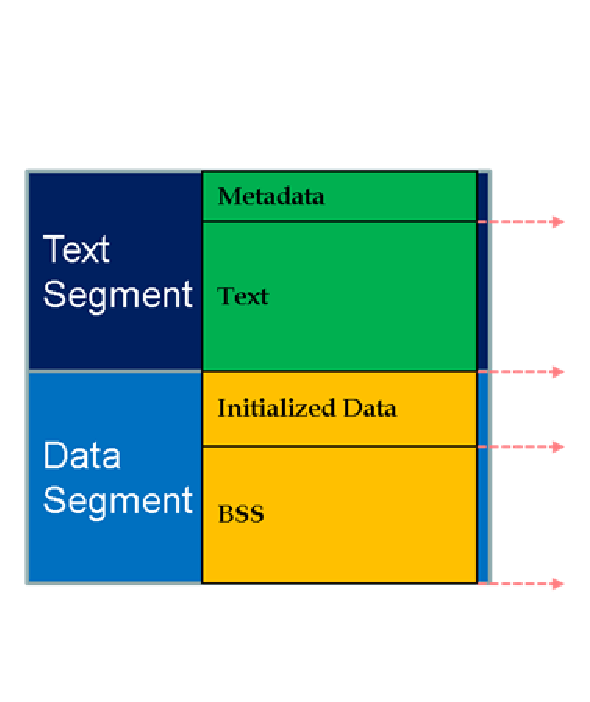
\includegraphics[scale=0.65]{executablep1.eps}
\label{Figure:OrigExecutable}
}
\subfigure[The two-segment structure of the ELF file once instrumentation code and data are inserted.]{
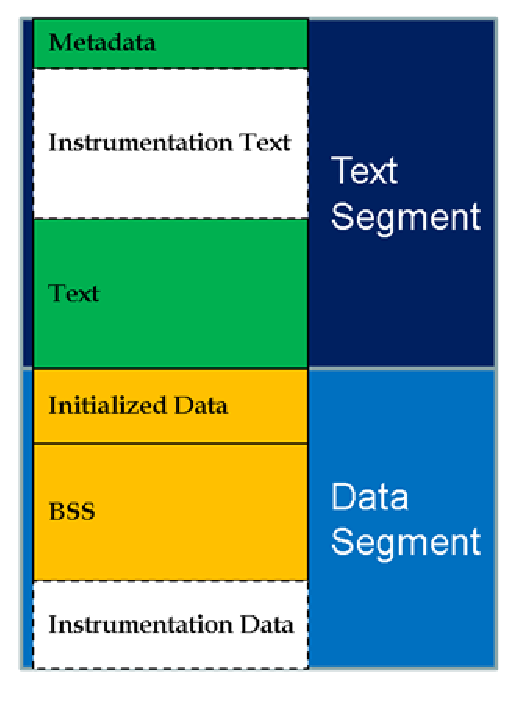
\includegraphics[scale=0.65]{executablep2.eps}
\label{Figure:InstExecutable}
}
\label{Figure:Executable}
\end{figure}

The instrumentation text contains several types of instrumentation code. The first
contains code that accomplishes the instrumentation task as well as some code to
accompany it. When control is transferred from the application to the
instrumentation code, it is necessary to maintain the machine state of
the application in order to preserve its original behavior. This machine state
can contain anything modified by the instrumentation code, but in practice is
usually limited to a relatively limited set of registers. The code snippet, called \textit{trampoline} [CITE Dyninst], 
saves any registers it intends to use, performs the instrumentation task, restores
any machine state after the instrumentation, executes the
original instructions that were displaced by the initial control transfer,
finally restoring control to the application. Since we are using an
unconditional branch instruction at the instrumentation point, at runtime the
instrumentation code has no information about where control was transferred from
(as might be the case if we used a more heavyweight call instruction). Hence
each instrumentation point uses its own trampoline so that the location of the
instrumentation point can be hard-coded into an unconditional branch instruction
at the end of the trampoline.

The instrumentation text also includes code to initialize data for use by the
instrumentation tool. Recall from Figure \ref{Figure:Executable} that the instrumentation
data was appended to the end of the application's data segment, after the
application's uninitialized data section  (BSS section). The initialized data and BSS
sections of the data segment are usually implemented by declaring the size of
the data segment in the executable to be smaller than the size of the data
segment in memory. According to the ELF[CITE] specification, the extra part of any
segment whose memory size is greater than its file size should be filled with
zeroes by the loader. Hence most programs just increase the size of the data
segment's size in memory by the size of the BSS section in order to get a large
area that is filled with zeroes and is reserved for uninitialized data. Since we
would like to use the area following the BSS section for (possibly initialized)
data for the instrumentation tool, we can either explicitly include the entire
segment's contents in the executable file or we can implicitly reserve this area
using the technique described above that is already in use by most programs.
Since the BSS section can be very large and explicit inclusion of its contents
would bloat the instrumented executable file unnecessarily, we use the implicit
technique to reserve this section for instrumentatoin data. We therefore
temporarily store the instrumentation data with the instrumentation text in the
executable, as well as some code to copy it to the appropriate location in the
data segment once the program starts.


\label{Section:Efficiency}
\section{Challenges}

\subsection{Relocation}
The novel use of relocation in our instrumentation strategy stems from the fact that we are performing
the instrumentation statically on a platform that uses a variable-length instruction
set. A typical strategy used by static instrumentation tools on platforms with 
fixed-length instruction sets is to replace a single fixed-length instruction at 
the instrumentation point with a branch instruction that will transfer control to 
the code produced by the instrumentation tool. This is fairly straightforward to
do because by the definition of a fixed-length instruction set,
the instruction being replaced and the replacement branch have the same length. Performing
static instrumentation in a variable-length instruction set does not afford us this luxury.
In X86, an unconditional branch that uses a 32-bit offset requires 5 bytes, whereas some
of the instrumentation points that interest us may use only a single byte.

This leaves two options for how to transfer control to the instrumentation code. We must either use 
a technique entirely distinct from the idea of using a single unconditional branch to execute the control
transfer such as multiple shorter jumps or software interrupts, or we must somehow alter the
application code so that it can accomodate a single large control instruction that is larger than the original
amount of space available at the instrumentation point. A seperate technique for transferring control flow
could be to use a series of branches, where the instruction in the instrumentation point is a small branch that
transfers control to a larger intermediate branch. We do not consider this method any further because the smallest
unconditional branch instruction is 2 bytes in length, making it ultimately a half measure since there are instrumentation
points with only a single byte available to them. Another option to consider is the method proposed by the BIRD project 
\ref{nanda2006bird}. They propose using the single-byte \begin{it}INT 3\end{it}
instruction, a single-byte interrupt intended to be used by debuggers to set breakpoints, when a larger branch won't fit within 
the specified area. This instructions is functionally perfect for static instrumentation because it consumes only a single
byte and allows us to transfer control to an arbitrary location by registering an exception handler
with the system. We performed a cursory study on this scheme from an efficiency standpoint to determine whether it was worth
further investigation. On a small benchmark set, our
implementation of using \begin{it}INT 3\end{it} only when 5-byte unconditional branches do
not fit at the instrumentation point introduces slowdowns of no less than 100-fold for counting the
number of executions of each basic block in the code. As one might expect, this mechanism is unsuitable
for efficient instrumentation because the very heavyweight system call conventions are being invoked
fairly often.

We use the latter option, reorganizing the code at the function level so that there is enough space at every instrumentation
point to accomodate a 5-byte branch. Specifically, the steps we use are as follows:
\begin{enumerate}
\item 
1. Function Displacement
\item
2. Link Function Entries 
\item
3. Branch Conversion
\item
4. Instruction Padding
\end{enumerate}


Figure \ref{Figure:Relocation} gives a visual version of this process.

1. Function Displacement: Relocate the contents of the entire function to an area of the text section allocated
to the instrumentation tool. Since functions are often packed tightly together, it is generally not possible to
expand the size of a function without disturbing the entry points of another function.

2. Link Function Entries: Place an unconditional branch at the former function entry point that transfers control
to the new function entry point. Most references to the entry point of a function are in the form of function calls, which
routinely are indirect references (ie their value is computed or looked up at runtime) and are difficult to resolve
prior to runtime.

3. Branch Conversion: Convert each short conditional branch in the relocated function to the equivalent
5-byte branch instruction. Since the code is being reorganized in the next step which may strain the limits of
smaller 8-bit or 16-bit offsets, we convert all branches to use 32-bit offsets so that the targets of each branch
will still be reachable without having the need to further reorganize the code. Note that there is some opportunity
here to reduce space by using the smallest branch offset size that accomodates the branch, but this is an issue
for future work.

4. Instruction Padding: According to the needs of the instrumentation tool, pad the instruction at each instrumentation
point with \begin{it}nop\end{it} instructions so that a 5-byte branch can fit.

There are several ways that this process can adversely affect the performance of the application independant of the overhead
that will be imposed by inserting any extra instrumentation code. Each function call
now has an extra control interruption associated with it since control must be passed first to the original function entry
point and then to the relocated function entry point. It is possible that using 32-bit offsets for every branch rather than
some smaller number of bits has an overhead associated with it. And since the code is being reorganized and expanded, 
we might destroy some positive alignment and size optimizations that the compiler might have made on the instructions in the
function. We examine the practical overhead seen by these techniques by taking these steps without instrumenting the code
for a series of benchmarks. The slowdown is XXXX...

\subsection{Disassembly Coverage}
Code and data can reside together in the text section of a program binary. This is done for a variety of reasons, including
the storage of branch target locations (eg for a jump table) or small data structures that provide convenient lookup
of certain data such as identifiers, descriptors, or other values.

Correctly determining
what parts of the text sections are code and what are data is important. Consider what can happen
if we mistakenly treat some data as code. We might choose to modify or relocate the apparent code
to serve our instrumentation purposes. Then when the data at this location is referenced, the
original program behavior may not be preserved: if we are lucky this will cause application failure
due to some unexpected change in control flow or some state condition that is checked by the program.
If we are unlucky the corruption might silently manifest itsself by modifying the output of the
program. Alternatively consider what can happen if we mistakenly treat some code as data. We then will
not try to insert code into this area or we might perform some other type of analysis that should be reserved for
data alone. While this is almost certainly preferrable to the situation where we treat data as code, it
is ideal to avoid both situations.

To this end, we use the program's symbol table to help us determine which parts of the text sections
are functions that are eligible to be subject for our code discovery algorithm. Our code discovery algorithm
consists of two phases; control-driven disassembly backed up by linear disassembly. In more detail, the algorithm
works as follows:

\begin{enumerate}
\item 
1. Control-driven disassembly: from a function's entry point, follow all understandable control paths. If a problem is encountered, fall back to
naive disassembly.
\item
2. Naive disassembly: from a function's entry point, disassemble each instruction in the order it appears in the
function. If a problem is encountered, give up.
\end{enumerate}


Problems that can be encountered are situations where an unknown opcode is encountered, where control jumps to the
middle of an instruction we've already disassembled, or if control leaves the boundaries of the function. In most
cases control-driven disassembly is sufficient to disassemble the entirety of a function, and in most cases control-driven
disassembly is a straightforward process because control either falls through to the following instruction 
or the location of a branch target is embedded entirely within the instruction itsself. But there are also cases
where the an indirect branch is used, where the target resides either at a fixed address (possibly with some offset), the address that resides in a register,
or the address that is at a location given by a register. The latter two cases are very difficult to resolve
without runtime information because the computation of the target address can be arbitrarily complex and can span function
boundaries. Nevertheless, we perform a peephole examination of the previous instructions to the and can determine 
the address in simple cases.

Fortunately simple calculations are all that most compilers use to determine targets for jump tables, one of the more common
uses of an indirect branch. Often an offset is added to a fixed location to determine where the data comprising the branch target
resides. Therefore we treat such a fixed address as the first entry in a table whose entries are treated either as addresses or as offsets.
We then make an iterative pass over this table to determine the target for each arm of the jump table, stopping when we find a value in the
table that yeilds an address that is outside the scope of the function.

PUT EXAMPLE OF GNU COMPILER JUMP TABLE HERE



\label{Section:Results}
\section{Results}
%\section{Results}
\label{sec:Results}

The main design goal of PEBIL is to generate efficient instrumented code. To
investigate the efficiency of instrumented executables created by PEBIL, we ran
several experiments on a selection of benchmarks from the the SPEC CPU2000
Integer benchmark suite comprised of bzip2, crafty, gap, gzip, mcf, parser,
perlmbk, twolf, vortex and vpr. All of the experiments are run on a single core
of a quad-core 2.4GHz IA32 Intel Xeon running Red Hat Linux Enterprise 4.1.2
(Linux kernel 2.6.18). 

The first set of experiments quantifies the overhead of the program relocation
and transformation techniques used by PEBIL as described in Section
\ref{Subsection:Relocation}. Recall that this technique adds an additional
unconditional branch execution to each function call in order to relocate the
function, extends all of the branches in the code to use 32-bit offsets, and
pads each basic block whose size is fewer than 5 bytes with nops so that a 5
byte jump to the instrumentation code can be inserted. These transformations were
performed on our benchmark set so that the code was ready for the insertion of
instrumentation code to measure the overhead caused by relocation and transformation. 

Figure \ref{fig:RelocOverhead} presents the runtime overhead seen in the
instrumentation-ready executables as a percentage of the original application
runtime. The figure shows that the maximum overhead due to these modifications
is 6.5\%, with an average overhead of just 1.6\%. Among a set of popular dynamic
instrumentation toolkits, Pin, DynamoRIO and Valgrind, the lowest overhead for
running the application within the instrumentation tool but performing no
instrumentation is obtained by using DynamoRIO. DynamoRIO has an average of 38\%
overhead and a maximum overhead of 113\% on the SPEC CPU2000 Integer benchmark
set \cite{luk2005pin}. This confirms that the relocation and transformation
method used by PEBIL has a minimal performance impact on the performance of
these benchmarks and thus is a suitable approach as a basis for producing
efficient instrumented code.

\begin{figure}[ht]
\centering
\label{fig:RelocOverhead}
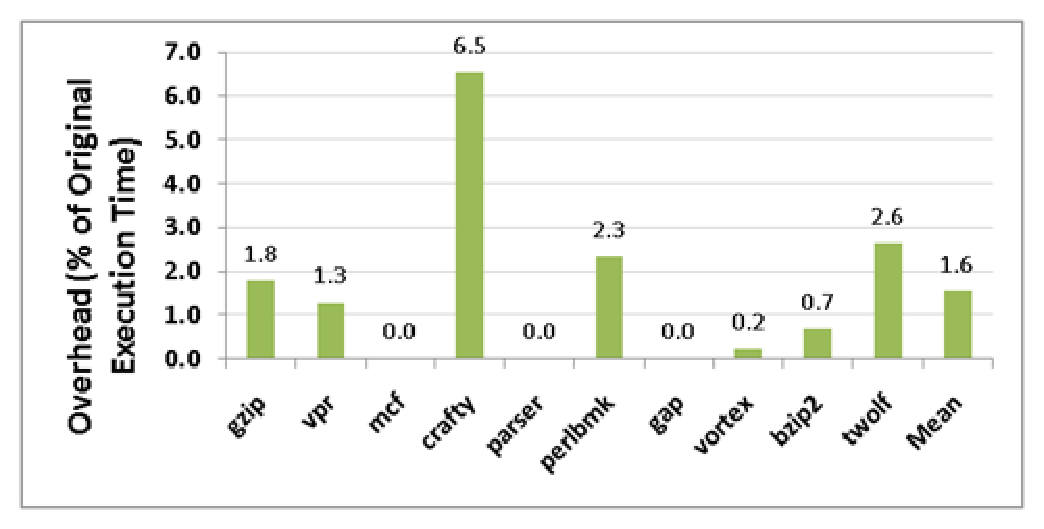
\includegraphics[scale=0.6]{relocperf.eps}
\caption{Application overhead caused by preparing the code for instrumentation but without
any instrumentation inserted.}
\end{figure}

The next set of experiments measure the overhead introduced due to counting the
basic block executions in the application. We use this particular
instrumentation tool because basic block counting is an example of an
instrumentation tool where we would expect PEBIL to generate efficient
instrumented executables since the number of instrumentation points required is
high. Much of the work performed in basic block counting, namely updating a
single counter every time a basic block is encountered, can be done easily using
a fast instrumentation snippet rather than by a full instrumentation function.
The counters embodied in the instrumentation snippets must also be persistent
throughout the entire run of the application, which is more suited to a static
instrumentation approach because the static instrumentation does not utilize any
resources to determine whether instrumentation can be removed. The basic block
counting instrumentation tool was used to produce an instrumented executable for
each program in our benchmark suite, whose runtime was compared to the runtime
of the unmodified original executable. The results of these experiments are
shown in Figure \ref{fig:ToolOverheads}. 

\begin{figure}[ht]
\centering
\label{fig:ToolOverheads}
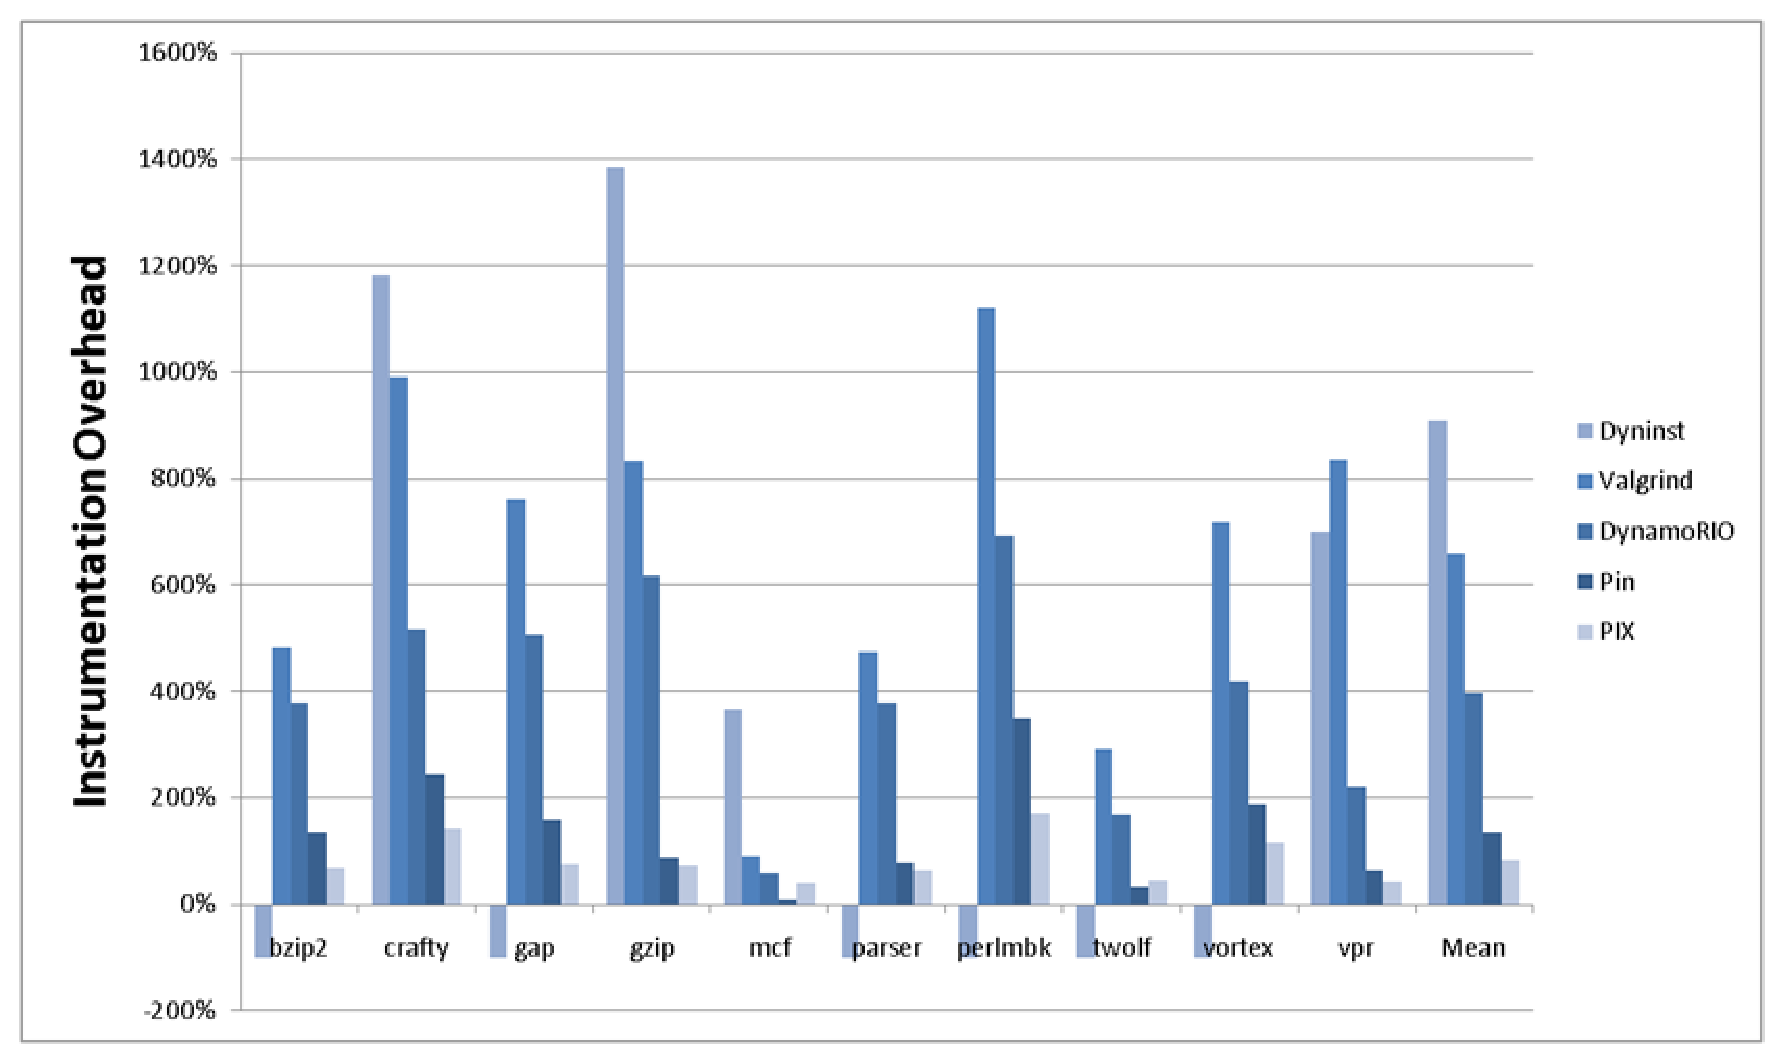
\includegraphics[scale=0.32]{bbcount.eps}
\caption{Performance of several x86 instrumentation tools with basic block counting instrumentation.}
\end{figure}

Figure \ref{fig:ToolOverheads} presents the overhead introduced as a percentage
of the original application runtime. The overhead of PEBIL's basic block counter
ranges from 41\%-170\% for the benchmarks tested with an average overhead of
84\%. More importantly, the figure shows that the overhead introduced by PEBIL
instrumentation is significantly lower than those introduced by the other
instrumentation toolkits available for the x86 platform. The average overhead is
135\% for Pin (ranging from 8\%-350\%), 396\% for DynamoRIO (ranging from
58\%-693\%), 660\% for Valgrind (ranging from 91\%-1120\%), and 1936\% for
Dyninst (ranging from 367\%-7859\%). Our experiments demonstrate that
executables instrumented by PEBIL run an average of 51\% faster than Pin, which
is the next most efficient instrumentation toolkit for basic block counting.
Furthermore, Pin uses a variety of optimizations such as tracking eflags bit
liveness \cite{luk2005pin} that are currently unincorporated into PEBIL. We plan
to incorporate more optimizations into PEBIL in the future (see Section
\ref{sec:Future}) including several optimizations already in use by Pin, which
should further improve the efficiency of the instrumented executables generated
by PEBIL.



\label{Section:Future}
\section{Future Work}
\label{sec:Future}

Despite the success in terms of efficiency, there are several additional techniques
that might make the instrumented code even more efficient in PIX. Because PIX relocates
the text to yeild extra space for the manipulation of the application functions, 
rather than inserting just a branch
that transfers control to the instrumentation code we have the opportunity to inline
the instrumentation code itsself
in order to reduce or eliminate the control interruptions  that otherwise must be taken 
when inserting the instrumentation code.

Currently PIX saves all general purpose registers around each function call and allows the
tool developer to state which registers are saved around instrumentation snippets. For even more efficient instrumentation
snippets, we could automatically detect which registers are killed by the instrumentation code and which are live at the entry point
of the instrumentation code, and automatically save only the ones that are alive. Similarly, we could perform register 
analysis in order to identify the instrumentation points where the machine state doesn't need to be saved around instrumentation functions. 

Finally, similar to Pin, we could perform liveness on the bits of the eflags/rflags register to determine whether the flag registers need to be saved and
restored at each instrumentation point. Optimizations that help PIX avoid saving and restoring state at each instrumentation point 
have the potential to further the overhead associated with instrumentation and we beleive 
that they will further the goal of generating efficient instrumented code with PIX.




\label{Section:Conclusions}
\section{Conclusions}
%\section{Conclusions}


\bibliography{x86inst}
\bibliographystyle{unsrt}

\end{document}

